\documentclass[12pt,a4paper,oneside]{report}
% ---------------------------------------------------------------------------
%  Noise-aware Unsupervised Anomalous Sound Detection (DCASE 2026 Task 2)
%  M.Tech CSE (AI and DS) AI Laboratory project report
% ---------------------------------------------------------------------------
\usepackage[utf8]{inputenc}
\usepackage[T1]{fontenc}
\usepackage{mathptmx}                 % Times-style text and mathematics
\usepackage[scaled=0.92]{helvet}
\usepackage{courier}
\usepackage[a4paper,top=3.0cm,bottom=3.0cm,left=2.8cm,right=2.8cm,headheight=15pt,headsep=0.8cm,footskip=1.2cm]{geometry}
\usepackage{graphicx,booktabs,array,longtable,float,caption,subcaption}
\usepackage{amsmath,amssymb}
\usepackage{enumitem}
\usepackage{setspace}
\usepackage{xcolor}
\usepackage{tikz}
\usetikzlibrary{calc,positioning}
\usepackage{eso-pic}
\usepackage{fancyhdr}
\usepackage{titlesec}
\usepackage{listings}
\PassOptionsToPackage{hyphens}{url}\usepackage{url}
\usepackage{xurl}
\usepackage[hidelinks]{hyperref}
\usepackage{microtype}

% ---- colours (restrained) --------------------------------------------------
\definecolor{inkblue}{RGB}{28,52,94}
\definecolor{rule}{RGB}{90,90,90}

% ---- page frame: thin double line on every page -----------------------------
\AddToShipoutPictureBG{%
  \begin{tikzpicture}[remember picture,overlay]
    \draw[line width=0.9pt,color=inkblue] ($(current page.south west)+(1.35cm,1.35cm)$) rectangle ($(current page.north east)+(-1.35cm,-1.35cm)$);
    \draw[line width=0.3pt,color=inkblue] ($(current page.south west)+(1.55cm,1.55cm)$) rectangle ($(current page.north east)+(-1.55cm,-1.55cm)$);
  \end{tikzpicture}}

% ---- headers and footers ---------------------------------------------------
\pagestyle{fancy}
\fancyhf{}
\fancyhead[L]{\small\itshape\nouppercase{\leftmark}}
\renewcommand{\chaptermark}[1]{\markboth{Chapter \thechapter.\ #1}{}}
\fancyhead[R]{\small DCASE 2026 Task 2}
\fancyfoot[C]{\small\thepage}
\renewcommand{\headrulewidth}{0.4pt}
\renewcommand{\footrulewidth}{0pt}
\fancypagestyle{plain}{\fancyhf{}\fancyfoot[C]{\small\thepage}\renewcommand{\headrulewidth}{0pt}}

% ---- headings --------------------------------------------------------------
\titleformat{\chapter}[display]{\normalfont\color{inkblue}}{\filright\large\scshape Chapter \thechapter}{0.6em}{\titlerule[0.6pt]\vspace{0.5em}\huge\bfseries\filright}[{\vspace{0.4em}\titlerule[0.6pt]}]
\titlespacing*{\chapter}{0pt}{0pt}{2.2em}
\titleformat{\section}{\large\bfseries\color{inkblue}}{\thesection}{0.8em}{}
\titleformat{\subsection}{\normalsize\bfseries}{\thesubsection}{0.8em}{}
\titlespacing*{\section}{0pt}{1.6em}{0.7em}
\titlespacing*{\subsection}{0pt}{1.2em}{0.5em}

% ---- captions, lists, spacing, listings ------------------------------------
\captionsetup{font=small,labelfont={bf,color=inkblue},width=0.92\textwidth,skip=6pt}
\setlist{nosep,leftmargin=*}
\onehalfspacing
\setlength{\parskip}{0.35em}
\graphicspath{{figures/}}
\lstset{basicstyle=\ttfamily\footnotesize,breaklines=true,frame=single,rulecolor=\color{rule},framesep=4pt,columns=fullflexible,keepspaces=true,xleftmargin=4pt}
\renewcommand{\arraystretch}{1.15}
\renewcommand{\topfraction}{0.85}\renewcommand{\bottomfraction}{0.6}\renewcommand{\textfraction}{0.1}\renewcommand{\floatpagefraction}{0.75}

% ======================= FILL IN BEFORE SUBMISSION =======================
\newcommand{\universityName}{Ahmedabad University}
\newcommand{\departmentName}{Department of Computer Science and Engineering}
\newcommand{\programmeName}{M.Tech. in Computer Science and Engineering (AI and Data Science)}
\newcommand{\courseName}{AI Laboratory}
\newcommand{\studentOne}{Rishita Vyas}
\newcommand{\studentOneId}{AU2644017}
\newcommand{\studentTwo}{Tamanna Khirshriya}
\newcommand{\studentTwoId}{AU2644031}
\newcommand{\supervisorName}{Maitrik Shah}
\newcommand{\academicYear}{2026--27}
\newcommand{\submissionMonth}{November 2026}
% ==========================================================================

\begin{document}

% ---------------------------- cover page ------------------------------------
\begin{titlepage}
\thispagestyle{empty}
\begin{center}
\vspace*{0.4cm}
{\large\scshape \universityName\par}
\vspace{0.3cm}
{\normalsize \departmentName\par}
\vspace{1.4cm}
{\color{inkblue}\rule{0.6\textwidth}{0.6pt}\par}
\vspace{0.9cm}
{\LARGE\bfseries Noise-aware Unsupervised Anomalous Sound Detection for Machine Condition Monitoring\par}
\vspace{0.8cm}
{\large DCASE 2026 Challenge -- Task 2\par}
\vspace{0.9cm}
{\color{inkblue}\rule{0.6\textwidth}{0.6pt}\par}
\vspace{1.3cm}
{\normalsize A project report submitted for the course\par}
{\large\itshape \courseName\par}
\vspace{0.3cm}
{\normalsize \programmeName\par}
\vspace{1.6cm}
\begin{tabular}{@{}p{0.52\textwidth}p{0.42\textwidth}@{}}
\multicolumn{2}{@{}l}{\textbf{Submitted by}}\\[4pt]
Part 1 -- Data, preprocessing and model training & \studentOne{} (\studentOneId)\\[4pt]
Part 2 -- Anomaly scoring, evaluation and application & \studentTwo{} (\studentTwoId)\\[12pt]
\textbf{Faculty supervisor} & \supervisorName\\
\end{tabular}
\vfill
{\normalsize Academic year \academicYear\par}
{\normalsize \submissionMonth\par}
\end{center}
\end{titlepage}

% ---------------------------- front matter ----------------------------------
\pagenumbering{roman}
\chapter*{Declaration}
\addcontentsline{toc}{chapter}{Declaration}
We declare that the work presented in this report was carried out by us as part of the \courseName{} course of the \programmeName{} programme. Part~1 (dataset audit, preprocessing, Autoencoder training and the handover package) was implemented by \studentOne{} and Part~2 (anomaly scoring, threshold calibration, evaluation and the demonstration application) by \studentTwo. All results reported here were produced by the submitted code on the DCASE 2026 Task~2 development data; every figure in the results tables was recomputed from the raw per-recording score files during a final audit. Sources used are cited in the references.

\vspace{1.5cm}
\noindent\begin{tabular}{@{}p{0.48\textwidth}p{0.48\textwidth}@{}}
\studentOne{} (\studentOneId) & \studentTwo{} (\studentTwoId)\\[1.2cm]
\rule{5cm}{0.4pt} & \rule{5cm}{0.4pt}\\
Signature and date & Signature and date
\end{tabular}

\chapter*{Abstract}
\addcontentsline{toc}{chapter}{Abstract}
Machines rarely fail, and when they do the sound they make is seldom something that has been recorded before. Anomalous sound detection therefore has to be learned from normal sound alone. This project builds and evaluates such a detector for the seven machine types of the DCASE 2026 Challenge Task~2 development dataset: ToyCar, ToyCar (Emu), Fan, Gearbox (Emu), Bearing (Emu), Slide Rail (Emu) and Valve (Emu). Every two-channel recording is converted into 128-band log-Mel spectrograms per channel, the two channels are concatenated, standardised and grouped into windows of five frames, and the resulting 1280-dimensional vectors are modelled by a fully connected Autoencoder with an eight-dimensional bottleneck. For each machine two models are trained on normal recordings only: Model~A on the 990 source-domain recordings and Model~B on the 990 source plus 10 target-domain recordings. A recording is scored by its reconstruction error, by the Mahalanobis distance of its latent codes, and by the Mahalanobis distance of its residual frames from the distribution of normal training data.

All fourteen models were trained, all 2\,800 test recordings were scored, and every reported metric was recomputed from the raw score files during a final audit without discrepancy. Averaged over the seven machines the strongest configuration is Model~B with residual Mahalanobis scoring (AUC 0.573, pAUC 0.537), with Model~B and reconstruction MSE close behind (AUC 0.568, pAUC 0.531). Latent-space Mahalanobis scoring does not separate anomalies (AUC 0.46). Detection is considerably easier in the source domain (AUC about 0.65) than in the target domain (AUC 0.44 to 0.50), and the ten target recordings improve the overall AUC in 16 of 21 machine-and-method combinations, though only by small amounts. Because the chosen protocol uses every normal recording for training, decision thresholds had to be calibrated on training scores; the report shows that this makes them optimistic, with 34 to 36\,\% of normal test recordings flagged instead of the intended 10\,\%. A Streamlit application performs single-file inference with the same saved models and code.


\tableofcontents
\listoffigures
\listoftables
\cleardoublepage
\pagenumbering{arabic}

% ---------------------------- chapters --------------------------------------
\chapter{Introduction}\label{ch:intro}
\section{Background}
Listening to a machine is one of the oldest ways of judging its health. An experienced operator can tell from a change in pitch or rhythm that a bearing is wearing or a valve is sticking, long before a sensor on the machine reports a fault. Microphones are inexpensive, need no contact with the machine and can listen continuously, which makes acoustic condition monitoring attractive for factories with many small machines. The difficulty is on the learning side. Failures are rare, their sounds are diverse, and the failure that matters most is usually one that has never been recorded. A detector therefore cannot be trained as a classifier of known faults; it has to learn what \emph{normal} sounds like and raise an alarm when a recording departs from it. This is the setting of unsupervised anomalous sound detection (ASD), which the DCASE Challenge has run as Task~2 since 2020 \cite{koizumi2020,dohi2023}.

The 2026 edition of the task \cite{dcase2026task2} is described as noise-aware. Each clip is recorded with two channels, and every machine type comes in two domains: a \emph{source} domain with plenty of normal training clips, and a \emph{target} domain, recorded under different conditions or background noise, for which only ten normal training clips are available. A useful detector must work in both domains even though it has seen almost nothing of the second one. This domain shift, rather than the modelling of normal sound itself, turned out to be the central difficulty in our results.

\section{What this project does}
We implemented a complete detector for all seven machine types of the development dataset, following the experimental plan given in the AI Laboratory problem statement:
\begin{enumerate}
  \item \textbf{Experiment~1} trains an Autoencoder on normal recordings and scores a test recording by its reconstruction error.
  \item \textbf{Experiment~2} replaces the reconstruction error by a Mahalanobis distance from the distribution of normal features, computed both in the Autoencoder's latent space and in its residual space, and compares the two scoring approaches.
  \item \textbf{Experiment~3} trains the same Autoencoder twice per machine, once on source-domain recordings only (Model~A) and once on source plus target recordings (Model~B), to measure what the ten target clips contribute.
\end{enumerate}
The work was split between the two of us. \studentOne{} (Part~1) audited the data, built the preprocessing and the Autoencoder, trained the fourteen models in Google Colab and prepared the statistics and handover package. \studentTwo{} (Part~2) scored the test recordings, calibrated thresholds, computed and compared the metrics and built the Streamlit application. Both parts share one library module, so training, evaluation and the application run byte-identical preprocessing and model code.

\section{How to read this report}
Chapters~\ref{ch:problem} to \ref{ch:env} describe the problem, the data as we actually found it, and the method and its implementation. Chapter~\ref{ch:results} presents the results, recomputed during a final audit from the per-recording score files. Chapters~\ref{ch:app} to \ref{ch:conclusion} describe the application, discuss what the results mean, state the limitations plainly and suggest what we would do next. The appendix lists folder structures, configuration values and the exact code interface used by Part~2.

\chapter{Problem Statement and Objectives}\label{ch:problem}
\section{Problem statement}
For each machine type we are given normal training recordings from a source domain (990 clips) and a target domain (10 clips). The task is to build a system that assigns an anomaly score to an unseen recording so that anomalous recordings receive higher scores than normal ones, in both domains. Anomalous recordings are available only in the test set and may be used for evaluation alone: never for training, model selection or threshold calibration. The problem statement fixes the representation (log-Mel spectrograms), the model family (an Autoencoder trained on normal data) and the three experiments listed in the introduction.

\section{Objectives}
\begin{enumerate}
  \item Audit the seven development archives and establish counts, domains, labels, sampling rate, channel count and duration from the files themselves rather than from the documentation.
  \item Implement one deterministic preprocessing and feature-extraction pipeline that treats both channels and is shared, unchanged, by training and inference.
  \item For every machine, train Model~A (990 source normals) and Model~B (990 source + 10 target normals) with the same architecture, optimiser, seed and epoch budget.
  \item Prepare the mean, covariance and regularised precision of normal latent codes and residual frames so that Mahalanobis scoring is possible without re-reading the training data.
  \item Score all test recordings with reconstruction MSE, latent Mahalanobis distance and residual Mahalanobis distance; calibrate thresholds without any test data; report AUC, pAUC, precision, recall and F1 overall and per domain.
  \item Compare Model~A with Model~B and the three scoring methods, per machine and on average.
  \item Deliver a reproducible code base with verification reports and a working demonstration application.
\end{enumerate}

\section{Division of work}
\begin{table}[!htb]\centering\footnotesize\renewcommand{\arraystretch}{1.25}
\begin{tabular}{@{}p{0.26\textwidth}p{0.68\textwidth}@{}}\toprule
\textbf{Part 1 -- \studentOne} & Archive inspection and full dataset audit; two-channel preprocessing and feature caching; Autoencoder implementation; training of the 14 models in a resumable Colab pipeline; Mahalanobis statistics; twelve-point model verification; handover package and library module. \\
\textbf{Part 2 -- \studentTwo} & Scoring of the 2\,800 test and 14\,000 calibration recordings; Gamma-based thresholds; binary predictions; AUC, pAUC, precision, recall and F1; model and method comparisons and graphs; Streamlit application. \\
\bottomrule\end{tabular}
\caption{Division of work between the two team members.}
\label{tab:division}
\end{table}

\chapter{Dataset}\label{ch:dataset}
\section{Source and organisation}
The development dataset \cite{dcase2026data} is distributed as one ZIP archive per machine type. Inside each archive a \texttt{train/} folder holds the normal training recordings of the source domain (990) and the target domain (10), and a \texttt{test/} folder holds 100 source-domain and 100 target-domain recordings, half normal and half anomalous in each domain. The file name carries everything we need to know about a clip, for example \texttt{section\_00\_source\_train\_} \texttt{normal\_0001\_\ldots.wav}: section, domain, split, label and index. One practical detail cost us some care. The folder name inside an archive is not the archive name; the archive \texttt{dev\_sliderEmu.zip}, for instance, unpacks to a folder called \texttt{sliderEmu}. The pipeline therefore reads the archive index and discovers the machine folder instead of assuming it.

\section{What the audit found}
Before anything was trained, every one of the $7\times1200$ recordings was opened; its sampling rate, channel count, duration and an MD5 digest were recorded in \texttt{dataset\_audit.csv} (8\,400 rows). Table~\ref{tab:dataset} summarises the outcome. All recordings are 16\,kHz two-channel WAV files, none was unreadable, and there were no duplicate names or duplicate contents. The problem statement describes clips of roughly eleven seconds; in the data the duration depends on the machine: 11\,s for ToyCar, 12\,s for ToyCar (Emu) and 10\,s for the other five. This matters later because the number of analysis windows per clip differs accordingly. The description of the dataset also mentions supplemental noise-only clips; none were present in the archives we audited, and none were used.

\begin{table}[!htb]
\centering
\caption{Audited development data per machine type (all 1200 recordings per machine opened; 16 kHz, 2 channels, no unreadable or duplicate files). Supplemental clips were not used.}
\label{tab:dataset}
\footnotesize
\renewcommand{\arraystretch}{1.18}
\resizebox{\textwidth}{!}{\begin{tabular}{lllrrrrrr}
\toprule
Machine & Archive & Folder & Src train & Tgt train & Test N/A src & Test N/A tgt & Dur. (s) & Supp. \\
\midrule
BearingEmu & dev\_bearingEmu.zip & bearingEmu & 990 & 10 & 50/50 & 50/50 & 10 & 0 \\
Fan & dev\_fan.zip & fan & 990 & 10 & 50/50 & 50/50 & 10 & 0 \\
GearboxEmu & dev\_gearboxEmu.zip & gearboxEmu & 990 & 10 & 50/50 & 50/50 & 10 & 0 \\
SlideRailEmu & dev\_sliderEmu.zip & sliderEmu & 990 & 10 & 50/50 & 50/50 & 10 & 0 \\
ToyCar & dev\_ToyCar\_r2.zip & ToyCar & 990 & 10 & 50/50 & 50/50 & 11 & 0 \\
ToyCarEmu & dev\_ToyCarEmu.zip & ToyCarEmu & 990 & 10 & 50/50 & 50/50 & 12 & 0 \\
ValveEmu & dev\_valveEmu.zip & valveEmu & 990 & 10 & 50/50 & 50/50 & 10 & 0 \\
\bottomrule
\end{tabular}}
\end{table}

A note on the two channels. The task description speaks of two microphones, but nothing in an individual file tells us which channel corresponds to which position, and a stereo file by itself does not prove that two physically separate microphones were used. Throughout this work the channels are therefore called Channel~1 and Channel~2 and are treated symmetrically.

\section{How the splits were used}
Under the protocol adopted for the experiments (Section~\ref{sec:protocol}) all 990 source normals train Model~A and all 1\,000 normals train Model~B. Nothing is held out, so there is no validation set. The 200 test recordings per machine were touched only in Part~2, and only to compute scores and metrics.

\chapter{System Architecture and Methodology}\label{ch:method}
\section{Overview}
Figure~\ref{fig:pipeline} shows the whole system in one line. A recording becomes a sequence of two-channel log-Mel frames; the frames are standardised with statistics that were stored inside the model checkpoint at training time; five consecutive frames are flattened into one 1280-dimensional window; the Autoencoder reconstructs each window and, on the way, produces an eight-dimensional latent code. From these quantities three scores are formed per window and averaged over the recording: the reconstruction mean squared error (Experiment~1), the squared Mahalanobis distance of the latent code, and the squared Mahalanobis distance of each 256-dimensional residual frame (Experiment~2). The recording is declared anomalous if its score exceeds a threshold calibrated on the scores of the training recordings.

\begin{figure}[!htb]\centering
\resizebox{\textwidth}{!}{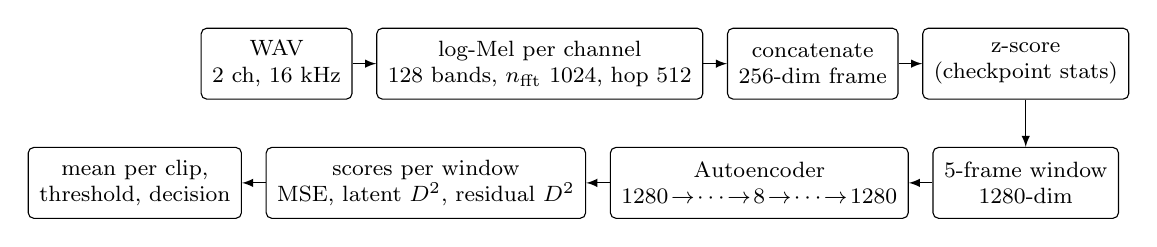
\begin{tikzpicture}[node distance=3mm,every node/.style={draw,rounded corners=2pt,align=center,font=\footnotesize,inner sep=4pt,minimum height=9mm,fill=white}]
\node (a) {WAV\\2 ch, 16 kHz};
\node (b) [right=of a] {log-Mel per channel\\128 bands, $n_\mathrm{fft}$ 1024, hop 512};
\node (c) [right=of b] {concatenate\\256-dim frame};
\node (d) [right=of c] {z-score\\(checkpoint stats)};
\node (e) [below=6mm of d] {5-frame window\\1280-dim};
\node (f) [left=of e] {Autoencoder\\$1280\!\to\!\cdots\!\to\!8\!\to\!\cdots\!\to\!1280$};
\node (g) [left=of f] {scores per window\\MSE, latent $D^2$, residual $D^2$};
\node (h) [left=of g] {mean per clip,\\threshold, decision};
\foreach \p/\q in {a/b,b/c,c/d,d/e,e/f,f/g,g/h} \draw[-latex] (\p) -- (\q);
\end{tikzpicture}}
\caption{Processing pipeline. The same code path is used for training, for scoring the test sets and inside the application.}
\label{fig:pipeline}
\end{figure}

\section{Relation to the official baseline}
Our design stays close to the official DCASE Autoencoder baseline \cite{harada2023}: the same spectral parameters, the same $128\times4\to8\to128\times4$ topology, 100 epochs, batch size 256, Adam with learning rate $10^{-3}$, no validation set, and scoring by MSE or Mahalanobis distance. We deviate in three ways, each of which is documented where it occurs. We use both channels (the baseline reads both but computes features from the first only); we standardise every feature dimension; and we compute Mahalanobis statistics in the latent space and in the 256-dimensional residual space rather than on 128-dimensional blocks of the raw reconstruction error. Because of these differences our numbers are not comparable with published baseline results, and we do not present them as such.

\section{Software structure}
Part~1 is one Google Colab notebook that processes the machines strictly one after another. It keeps a state file and a completion marker for every step, so that a disconnected session can be resumed by simply running the notebook again. At the end it writes the folder tree reproduced in Appendix~\ref{app:folders} and a verified handover archive. The functions that define preprocessing, the model and inference are collected in a module, \texttt{dcase\_part1\_lib.py}, that the notebook generates from its own cells. The Part~2 scripts and the Streamlit application import this module, which is how we guarantee that a recording scored in the application is processed exactly as it was during evaluation.

\chapter[Audio Preprocessing and Features]{Audio Preprocessing and Feature Extraction}\label{ch:prep}
\section{From waveform to feature window}
The preprocessing is deliberately plain, because it has to behave identically in three places: when features are cached for training, when Part~2 scores a test file, and when a user uploads a recording to the application. The steps are:
\begin{enumerate}
  \item Load the WAV file with \texttt{soundfile} as 32-bit floating point, keeping both channels.
  \item Resample a channel only if its rate differs from 16\,kHz. In practice this branch never ran, since every audited file is already at 16\,kHz.
  \item Compute, for each channel, a Mel power spectrogram with \texttt{librosa} \cite{librosa}, using an FFT length of 1024 samples (64\,ms), a hop of 512 samples (50\,\%), 128 Mel bands and power~2, and convert it to decibels with the same formula as the official baseline,
  \begin{equation}
    X_{t,m} = \frac{20}{p}\,\log_{10}\!\big(\max(S_{t,m},\varepsilon)\big), \qquad p = 2,\quad \varepsilon = 2.2\times 10^{-16},
    \label{eq:logmel}
  \end{equation}
  where $S_{t,m}$ is the Mel power in frame $t$ and band $m$.
  \item Concatenate the two 128-band frames of the same time step into one 256-dimensional frame, and replace any non-finite value.
  \item Standardise each of the 256 dimensions with the mean $\mu_m$ and standard deviation $\sigma_m$ computed over the training frames of the model in use: $\tilde X_{t,m} = (X_{t,m}-\mu_m)/\sigma_m$. These statistics are stored in the checkpoint, so inference never needs the training data.
  \item Form overlapping windows of five consecutive frames (stride one) and flatten each to a 1280-dimensional vector.
\end{enumerate}
A 10\,s clip gives 309 windows, an 11\,s clip 340 and a 12\,s clip 372. We neither pad nor crop clips of different lengths; the model sees windows, so a longer clip simply contributes more of them. Features of all training recordings are extracted once per machine and cached, which made the fourteen training runs considerably faster than re-reading the audio each epoch would have been.

\section{Why both channels, and why standardise}
We kept both channels because the difference between the two domains in this task lies in the acoustic conditions, and whatever the second channel adds about the surrounding noise is exactly the information a noise-aware detector should see. Concatenating the two channels was the least intrusive way to use them: the Autoencoder needs a wider first and last layer and nothing else changes.

Standardisation is the other departure from the baseline. Raw log-Mel values span tens of decibels and differ systematically between low and high bands, so without standardisation the reconstruction loss is dominated by the loudest bands and by the overall decibel offset. An early single-machine prototype that trained on unnormalised features produced losses in the hundreds that said little about how well the model was doing. With per-dimension z-scoring every band carries comparable weight and the losses, shown in Figure~\ref{fig:losses}, are of order one.

\begin{figure}[!htb]\centering
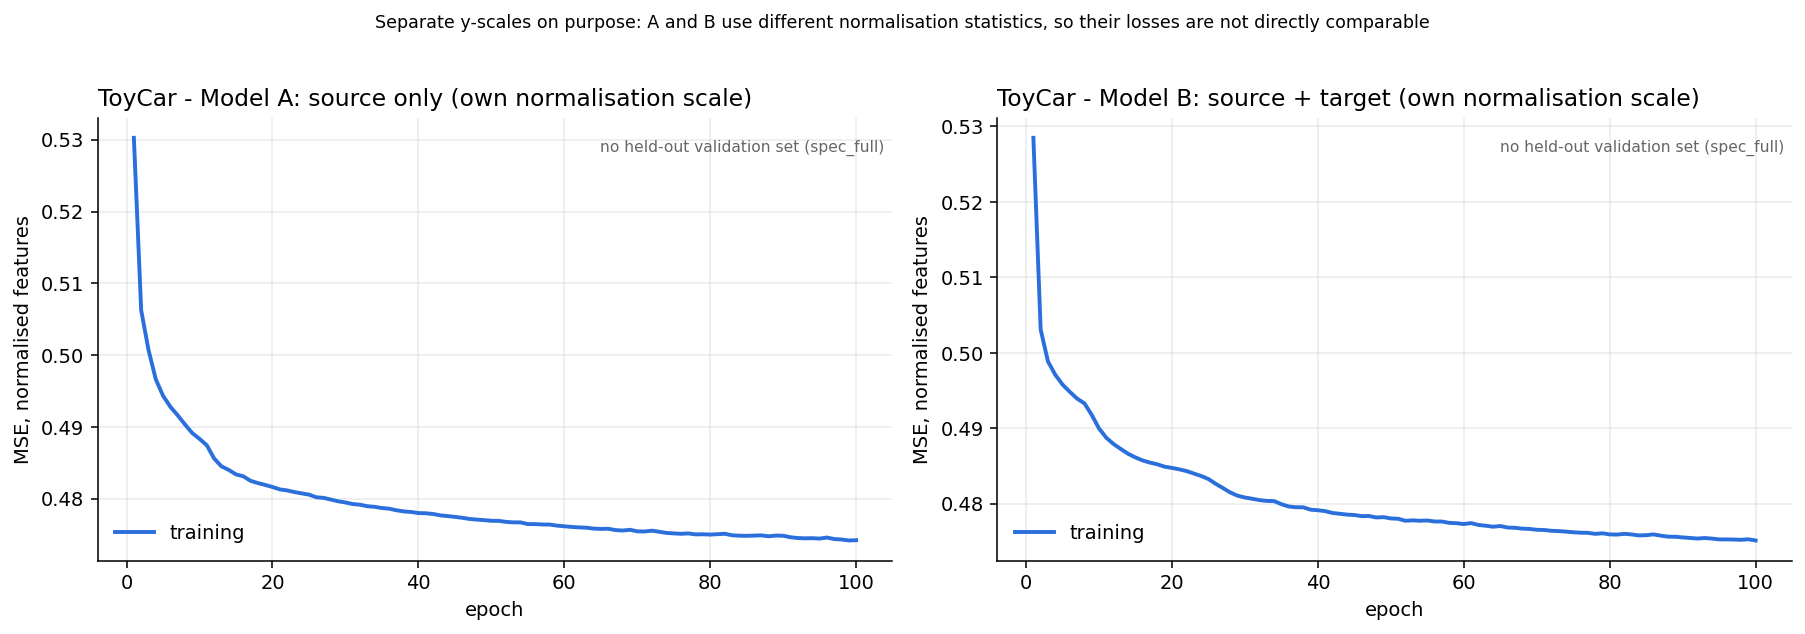
\includegraphics[width=0.9\textwidth]{ToyCar_training_curves_per_model}
\caption{Training loss of the two ToyCar models, Model~A on the left and Model~B on the right. Each panel is on its own normalisation scale. The annotation records that no held-out validation set exists under the adopted protocol.}
\label{fig:toycarloss}
\end{figure}

\chapter{Autoencoder Architecture}\label{ch:ae}
The model is a symmetric fully connected Autoencoder:
\begin{equation}
1280 \;\to\; 128 \;\to\; 128 \;\to\; 128 \;\to\; 128 \;\to\; \underbrace{8}_{\text{latent } z} \;\to\; 128 \;\to\; 128 \;\to\; 128 \;\to\; 128 \;\to\; 1280 .
\label{eq:topology}
\end{equation}
Every hidden layer is followed by batch normalisation and a ReLU; the output layer is linear so that it can reproduce standardised values of either sign. The network has 432\,408 trainable parameters. For an input window $x \in \mathbb{R}^{1280}$ the encoder produces the code $z = f_\theta(x) \in \mathbb{R}^{8}$ and the decoder the reconstruction $\hat{x} = g_\phi(z)$. Training minimises the mean squared reconstruction error over all training windows,
\begin{equation}
\mathcal{L}(\theta,\phi) = \frac{1}{N}\sum_{i=1}^{N} \frac{1}{1280}\,\lVert x_i - \hat{x}_i \rVert_2^2 .
\label{eq:loss}
\end{equation}
The optimiser is Adam with learning rate $10^{-3}$, batch size 256 and random seed 42, for a fixed budget of 100 epochs.

The topology is that of the official baseline \cite{harada2023}; only the input and output width follow our 1280-dimensional two-channel features instead of the baseline's 640. One Python class, \texttt{DCASEAutoencoder}, serves all fourteen models, and its \texttt{forward} method returns both $\hat{x}$ and $z$. That small choice is what lets Part~2 score in the latent space without touching the model.

An eight-dimensional bottleneck is a strong compression of a 1280-dimensional window. The idea behind using it for anomaly detection is that the decoder can only rebuild patterns it has seen during training; a window that contains an unfamiliar sound should therefore come back distorted, and the distortion is the anomaly signal. Whether the bottleneck itself also places unfamiliar windows at unusual positions in $z$-space is an empirical question, and Experiment~2 answers it.

\chapter[Experiment 1: Autoencoder Training and MSE Scoring]{Experiment 1: Autoencoder Training and Reconstruction-based Scoring}\label{ch:exp1}
\section{Purpose}
Experiment~1 establishes the reference detector: an Autoencoder trained on normal recordings only and used through its reconstruction error. Everything else in the project builds on the fourteen models trained here, so this chapter also fixes the training protocol and documents how the training was actually run.

\section{Training protocol}\label{sec:protocol}
The problem statement specifies that Model~A uses the 990 source-domain recordings and Model~B the 990 source plus 10 target recordings. We followed this literally: each model is trained on \emph{all} the normal recordings of its configuration, a protocol we call \texttt{spec\_full} in the code. The consequence has to be stated clearly, because it shapes the rest of the report. Since no recording is held out, there is no validation set, no validation loss and no early stopping; the checkpoint after the hundredth epoch is the model. This is also what the official baseline does. The training-loss curve is monitored for convergence (Figure~\ref{fig:losses}) and snapshots are kept every ten epochs, but nothing in the training procedure can detect overfitting. An alternative protocol with a 10\,\% hold-out was implemented in the notebook for an earlier single-machine prototype; it was not used for any of the models reported here.

\section{How the training was run}
All fourteen models were trained on 9~November~2026 in a single Google Colab session with a CUDA GPU runtime. The session log records \texttt{device=cuda} at start, and every checkpoint stores \texttt{device: cuda} together with its start and finish time. The machines were processed one after another from 16:48 to 20:06 UTC, a total of 3\,h\,17\,min including archive extraction, the full audit and feature caching; the per-model training times in Table~\ref{tab:training} add up to 186.5 minutes. A second Colab session on 10~November ran on a CPU runtime and did nothing but re-assemble and verify the handover archive, which is why the environment file written last records \texttt{device: cpu}. No model was trained or modified in that session. The GPU model itself is not recorded in the logs, so we do not name one.

\begin{table}[!htb]
\centering
\caption{Training summary for the 14 models (spec\_full protocol: fixed 100 epochs, final-epoch checkpoint, no validation set). Training executed on a CUDA GPU in Google Colab on 9 November 2026.}
\label{tab:training}
\footnotesize
\renewcommand{\arraystretch}{1.18}
\resizebox{\textwidth}{!}{\begin{tabular}{lrrrrrrr}
\toprule
Machine & Model & Source rec. & Target rec. & Train windows & Epochs & Final train MSE & Minutes \\
\midrule
ToyCar & A & 990 & 0 & 336600 & 100 & 0.474 & 14.600 \\
ToyCar & B & 990 & 10 & 340000 & 100 & 0.475 & 13.000 \\
ToyCarEmu & A & 990 & 0 & 368280 & 100 & 0.496 & 16.300 \\
ToyCarEmu & B & 990 & 10 & 372000 & 100 & 0.496 & 14.400 \\
Fan & A & 990 & 0 & 305910 & 100 & 0.729 & 13.700 \\
Fan & B & 990 & 10 & 309000 & 100 & 0.731 & 11.900 \\
GearboxEmu & A & 990 & 0 & 305910 & 100 & 0.376 & 13.600 \\
GearboxEmu & B & 990 & 10 & 309000 & 100 & 0.377 & 11.900 \\
BearingEmu & A & 990 & 0 & 305910 & 100 & 0.472 & 13.700 \\
BearingEmu & B & 990 & 10 & 309000 & 100 & 0.472 & 12.000 \\
SlideRailEmu & A & 990 & 0 & 305910 & 100 & 0.465 & 13.700 \\
SlideRailEmu & B & 990 & 10 & 309000 & 100 & 0.464 & 12.000 \\
ValveEmu & A & 990 & 0 & 305910 & 100 & 0.522 & 13.700 \\
ValveEmu & B & 990 & 10 & 309000 & 100 & 0.522 & 12.000 \\
\bottomrule
\end{tabular}}
\end{table}

The final training losses in Table~\ref{tab:training} range from 0.38 (Gearbox Emu) to 0.73 (Fan). We read these only as a sign that each model converged; because A and B standardise their features with slightly different statistics, the two losses of one machine are not a ranking of the two models, and the test-set metrics of Chapter~\ref{ch:results} are the only basis for comparing them.

\section{Reconstruction-error score}
For a test recording with windows $x_1,\dots,x_W$ the Experiment~1 anomaly score is the average window error,
\begin{equation}
s_\mathrm{MSE} = \frac{1}{W}\sum_{w=1}^{W} \frac{1}{1280}\,\lVert x_w - \hat{x}_w \rVert_2^2 .
\label{eq:mse}
\end{equation}

\section{Verification}
Each checkpoint was put through twelve checks before it was accepted: the file exists and loads; the architecture and parameter count are as expected; input, output and latent dimensions are correct; a forward pass on random data and on genuine recordings produces no NaN or infinite values; two inference runs on the same input give identical results; the saved normalisation statistics load and equal those in the checkpoint; and the Mahalanobis statistics of Experiment~2 are valid and correctly shaped. All fourteen models passed (\texttt{ALL\_MACHINES\_verification\_summary.csv}).

\begin{figure}[!b]\centering
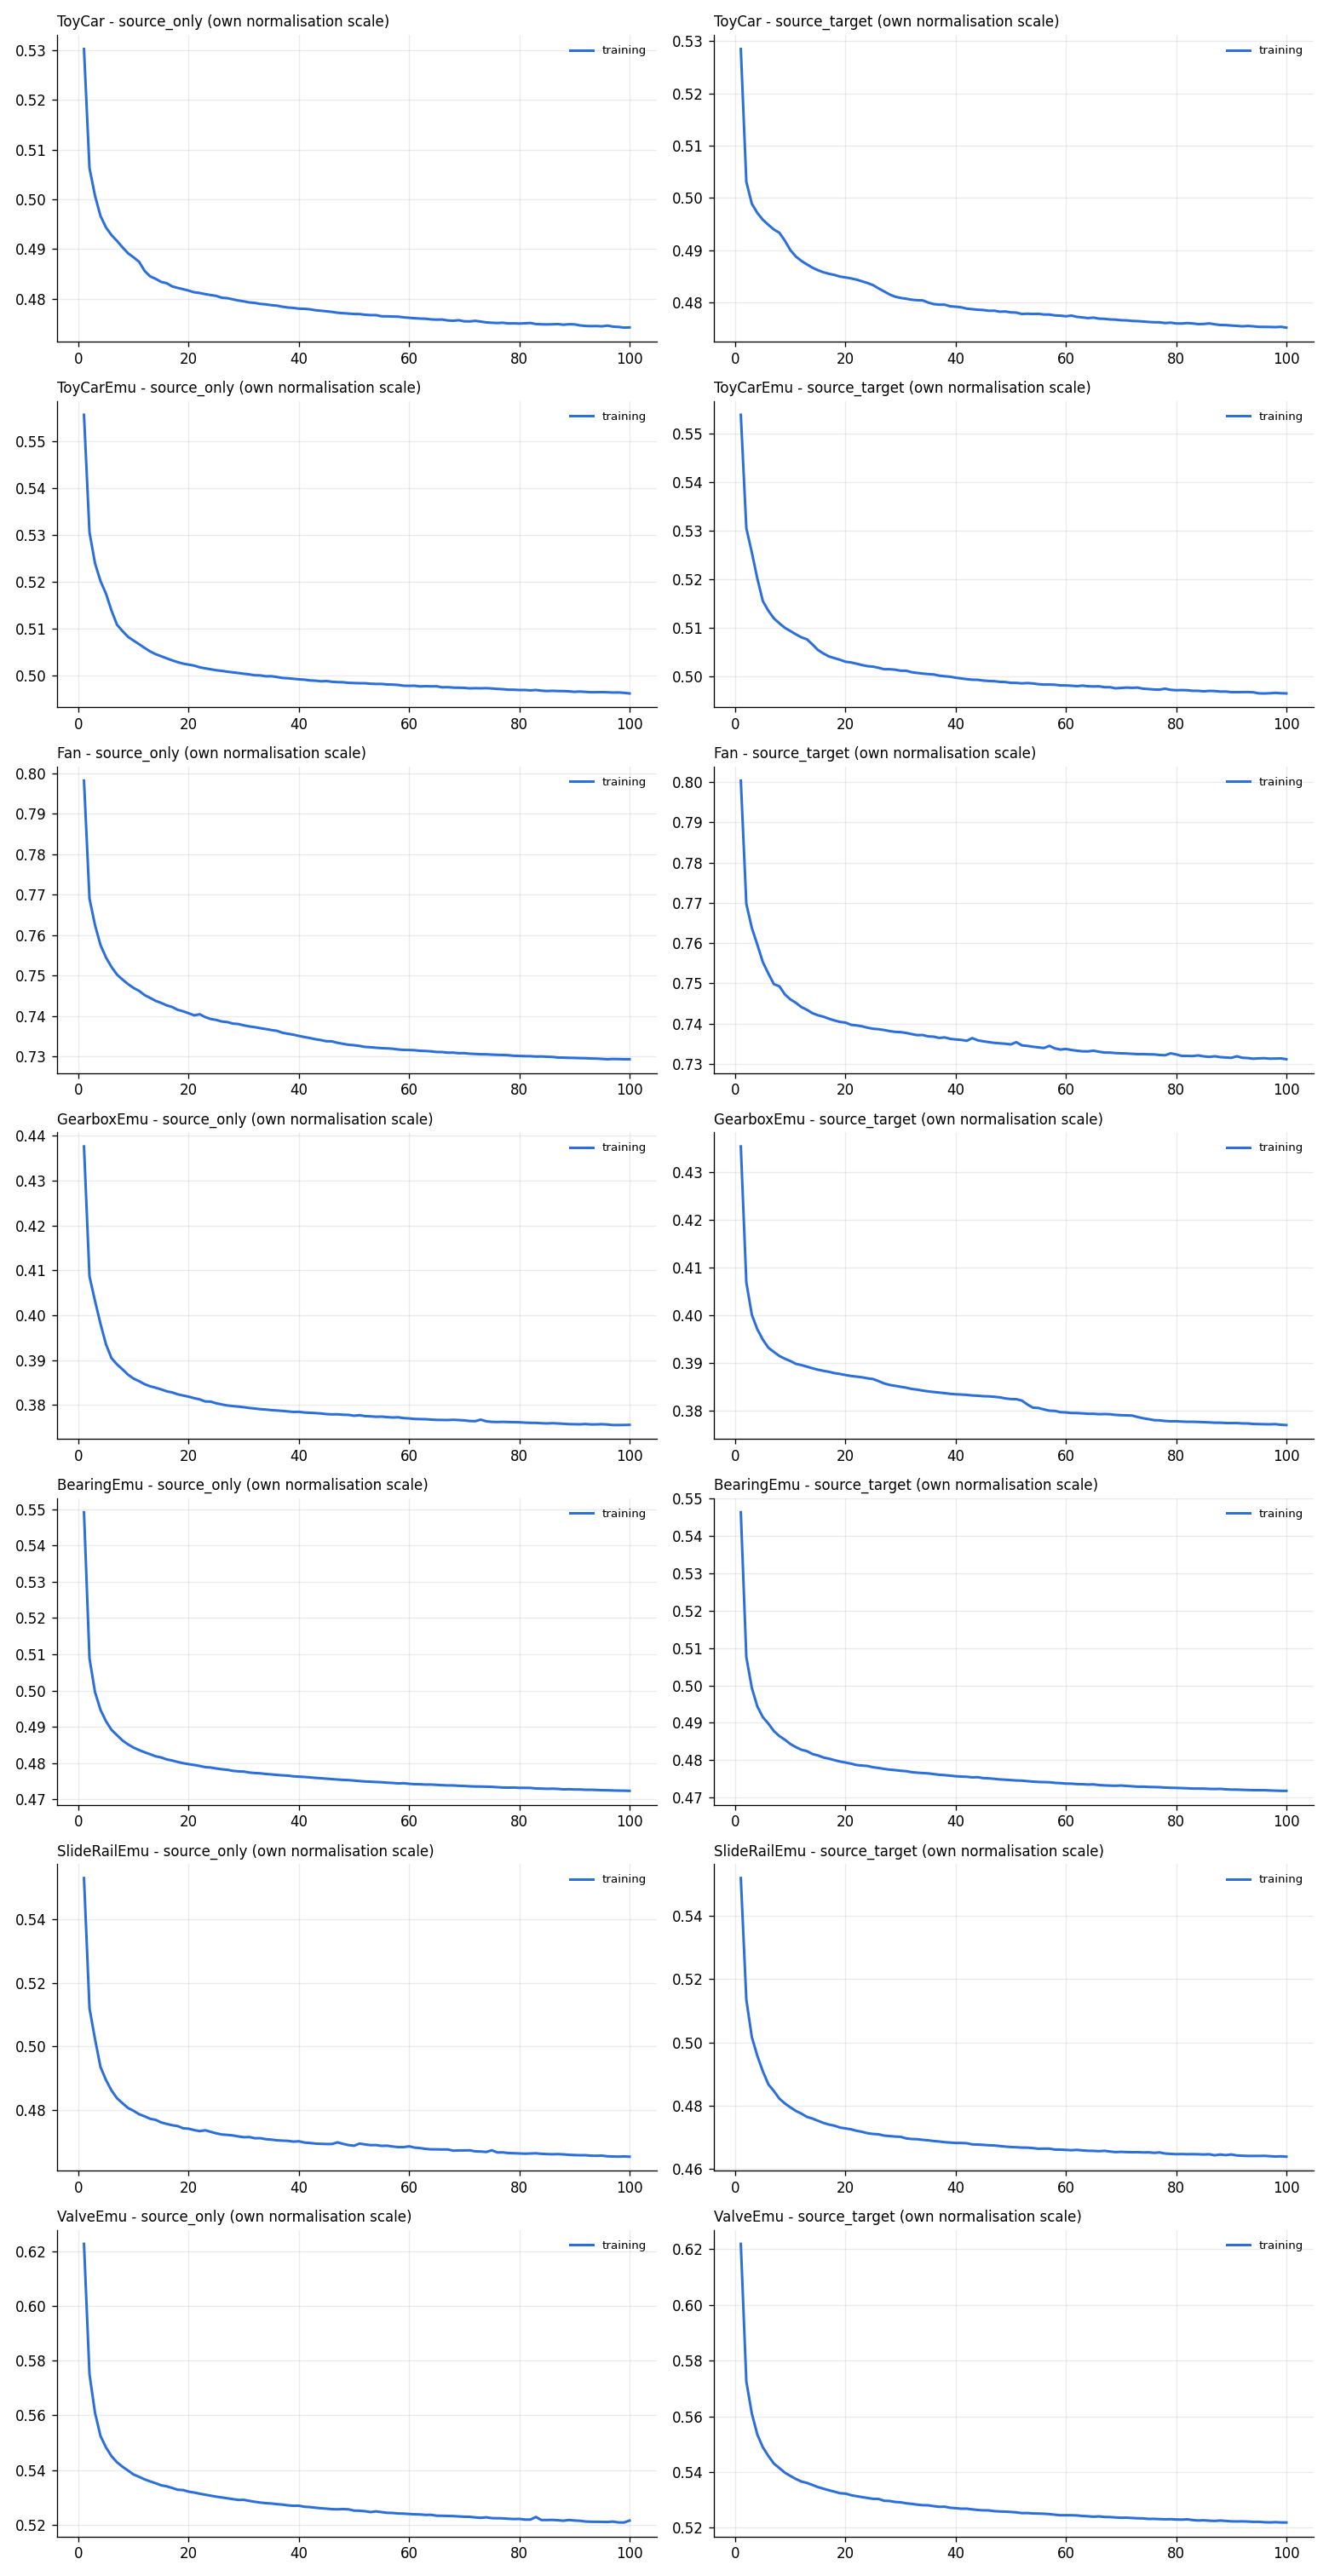
\includegraphics[width=0.96\textwidth,height=0.74\textheight,keepaspectratio]{ALL_MACHINES_loss_curves}
\caption{Training-loss curves of all fourteen models. Rows are machines; the left column is Model~A, the right column Model~B. Each curve is the mean squared error on that model's own standardised features, so values are not comparable across panels.}
\label{fig:losses}
\end{figure}

\chapter{Experiment 2: Mahalanobis-distance Scoring}\label{ch:exp2}
\section{Purpose}
Reconstruction error treats every one of the 1280 output values alike. Some bands, however, are always reconstructed poorly even for normal sound, while others are reconstructed almost perfectly, and an error in the second kind of band is far more telling than an error in the first. Experiment~2 asks whether a distance that accounts for this structure, the Mahalanobis distance from the distribution of normal features, detects anomalies better than the plain MSE. We apply it in two feature spaces: the eight-dimensional latent code, which tests whether anomalies are mapped to unusual codes, and the 256-dimensional residual frame, which reweights the reconstruction error by its normal variability.

\section{Statistics of normal data}
After training, Part~1 passes every training window of a model through the network once more and accumulates, in double precision, the mean $\mu$ and covariance $\Sigma$ of the latent codes $z$ and of the residual frames $r = x - \hat{x}$ reshaped to one 256-dimensional row per frame. This is done for three groups of normal training recordings: \texttt{source\_train} (990 source normals), \texttt{target\_train} (the 10 target normals) and \texttt{all\_train} (all 1\,000). No \texttt{validation\_source} group exists, since the protocol holds nothing out. The covariance is regularised and inverted as
\begin{equation}
\Sigma_\mathrm{reg} = \Sigma + \lambda I, \qquad \lambda = 10^{-3}\,\frac{\operatorname{tr}\Sigma}{d}, \qquad P = \Sigma_\mathrm{reg}^{-1},
\label{eq:reg}
\end{equation}
where $d$ is 8 or 256 and the inverse is obtained by a Cholesky solve. The relative choice of $\lambda$ keeps it meaningful whatever the scale of the features; the Cholesky factorisation doubles as a proof that $\Sigma_\mathrm{reg}$ is positive definite. For every one of the 84 statistic files the pipeline records dimensions, smallest eigenvalue, condition number, inverse error and sample count, and all passed.

\section{Mahalanobis scores}
The squared Mahalanobis distance \cite{mahalanobis1936} of a vector $v$ from the normal distribution of its group is
\begin{equation}
D^2(v) = (v-\mu)^{\top} P\,(v-\mu).
\label{eq:maha}
\end{equation}
The \emph{latent} score of a recording is the average of $D^2(z_w)$ over its $W$ windows; the \emph{residual} score is the average of $D^2(r)$ over all $5W$ residual frames. Part~2 scores each model against the statistics of the recordings it was trained on, \texttt{source\_train} for Model~A and \texttt{all\_train} for Model~B; the distances to all three groups were nevertheless stored in the score files for later analysis. It is worth keeping the two kinds of score apart in one's mind: MSE measures how badly a window is rebuilt, whereas the Mahalanobis distance measures how far a feature vector lies from where normal feature vectors lie, after correcting for their correlations.

\section{Threshold calibration}
To turn a score into a decision we followed the official baseline. For each machine, model and scoring method the scores of the model's own training normals (990 for Model~A, 1\,000 for Model~B) are collected, a Gamma distribution with location fixed at zero is fitted by maximum likelihood, and its 90th percentile becomes the threshold. This gives 42 thresholds, stored with their fitted parameters and the empirical 90th percentile. We want to be explicit about what this does and does not achieve. No test recording and no test label influenced any threshold. But the calibration recordings are the ones the model was trained on, and a model reconstructs what it has fitted better than what it has not; their scores are therefore systematically lower than those of unseen normal recordings, and a threshold set from them is optimistic. This is not an oversight that could have been avoided within the protocol: once every normal recording is used for training, there is no independent normal recording left to calibrate on. Section~\ref{sec:rates} measures the size of the effect.

\chapter[Experiment 3: Source-only versus Source + Target]{Experiment 3: Source-only versus Source\,+\,Target Training}\label{ch:exp3}
\section{Purpose}
Only ten target-domain recordings are available for training, about one percent of the training set. Experiment~3 asks a simple question: does including them help the detector in the target domain, and does it cost anything in the source domain?

\section{Design}
For every machine the same architecture, preprocessing, optimiser, seed and epoch budget are used twice. Model~A is trained on the 990 source normals, Model~B on the 990 source normals plus the 10 target normals. Each model computes its standardisation statistics from its own training set, so the ten target clips influence Model~B in two ways: through the gradient updates and, slightly, through the feature scaling. Both models are then scored with all three methods on the identical 200 test recordings of each machine and compared with the same metrics in Chapter~\ref{ch:results}. We deliberately do not compare the two models by their training loss. Their losses are measured on differently standardised features, and in any case a lower reconstruction error on normal sound says nothing about how well anomalies are separated.

\chapter{Implementation Environment}\label{ch:env}
\begin{table}[!htb]\centering\footnotesize\renewcommand{\arraystretch}{1.3}
\begin{tabular}{@{}p{0.3\textwidth}p{0.64\textwidth}@{}}\toprule
\textbf{Part 1 model training} & Google Colab, CUDA GPU runtime, 9 November 2026, 16:48 to 20:06 UTC. Evidence: \texttt{device=cuda} in the session log and \texttt{device: cuda} with start and finish times in all 14 checkpoints. GPU model not recorded. \\
\textbf{Part 1 handover verification} & Google Colab, CPU runtime, 10 November 2026 (Python 3.13.18, PyTorch 2.14.1+cpu, librosa 0.11.0, soundfile 0.14.0, NumPy 2.4.6, SciPy 1.16.3, scikit-learn 1.6.1). This session only re-assembled and verified the handover archive; it is the session recorded in \texttt{environment.json}. \\
\textbf{Part 2 scoring, thresholds, metrics, application} & Windows laptop, Python 3, PyTorch on CPU, librosa, soundfile, SciPy, scikit-learn, Streamlit. \\
\textbf{Persistent storage} & Google Drive folder \texttt{DCASE\_2026\_PART1\_COMPLETE/}; handover archive of 225 files, 55.3\,MB. \\
\textbf{Reproducibility} & Seed 42 for Python, NumPy and PyTorch; all configuration values stored in \texttt{common\_config.json} and inside every checkpoint. \\
\bottomrule\end{tabular}
\caption{Implementation environment. The training session and the later verification session ran on different hardware and are listed separately.}
\label{tab:env}
\end{table}

The Colab notebook was written to survive the interruptions that free Colab sessions suffer: every epoch writes a resume checkpoint, every finished experiment a completion marker, and a pipeline state file tracks each machine, so a second run continues where the first stopped. As it happened, the training session of 9~November ran to completion without interruption, which the continuous timestamps in \texttt{logs/part1\_master.log} confirm.

\chapter{Results and Evaluation}\label{ch:results}
\section{Metrics and how they were checked}
AUC is the area under the ROC curve over all 200 test recordings of a machine. pAUC is the partial area for false-positive rates up to 0.1, normalised to the range $[0,1]$ (scikit-learn's \texttt{roc\_auc\_score} with \texttt{max\_fpr=0.1}), and rewards methods that catch anomalies before they start raising many false alarms. The domain AUCs follow the DCASE convention: the normal recordings of one domain are compared against \emph{all} anomalous recordings, so that a model which merely scores one domain higher than the other is not rewarded. Precision, recall and F1 are computed within each domain at the calibrated threshold.

Every number in this chapter was recomputed during the final audit from the per-recording score and prediction files, independently of the scripts that first produced it. The recomputed thresholds agree with the delivered ones to a relative difference of $2\times10^{-14}$, all 8\,400 decisions follow from their thresholds, and the recomputed metrics agree with \texttt{all\_machine\_metrics.csv} to $8\times10^{-17}$.

\section{Average results}
\begin{table}[!htb]
\centering
\caption{Metrics averaged over the seven machine types (test sets, 200 recordings each). AUC src/tgt follow the DCASE definition (domain normals versus all anomalies). F1 uses the Gamma 90th-percentile threshold fitted on training-set scores.}
\label{tab:average}
\footnotesize
\renewcommand{\arraystretch}{1.18}
\begin{tabular}{lrrrrrrr}
\toprule
Model & Scoring & AUC & pAUC & AUC src & AUC tgt & F1 src & F1 tgt \\
\midrule
A & MSE & 0.547 & 0.516 & 0.658 & 0.436 & 0.398 & 0.451 \\
A & Lat.\,Mah. & 0.466 & 0.494 & 0.473 & 0.459 & 0.120 & 0.085 \\
A & Res.\,Mah. & 0.557 & 0.530 & 0.653 & 0.460 & 0.450 & 0.441 \\
B & MSE & 0.568 & 0.531 & 0.653 & 0.484 & 0.403 & 0.468 \\
B & Lat.\,Mah. & 0.457 & 0.491 & 0.485 & 0.429 & 0.125 & 0.121 \\
B & Res.\,Mah. & 0.573 & 0.537 & 0.650 & 0.496 & 0.444 & 0.449 \\
\bottomrule
\end{tabular}
\end{table}
\begin{figure}[!htb]\centering
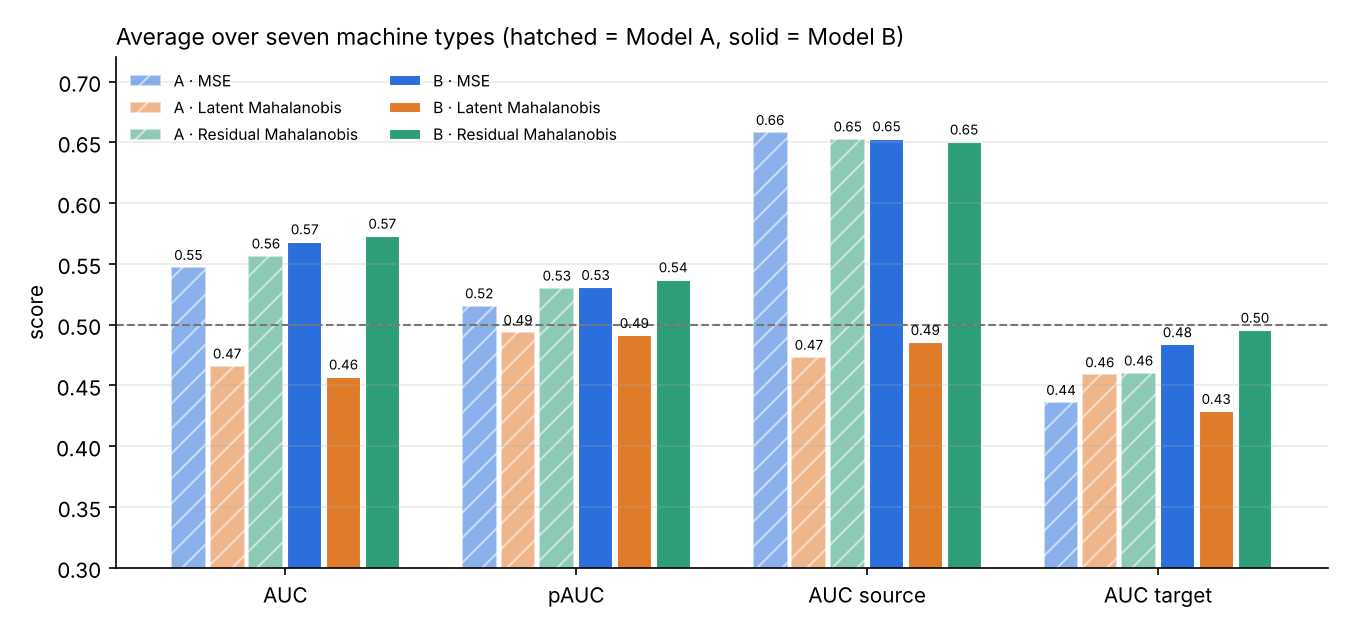
\includegraphics[width=0.95\textwidth]{fig_average_comparison}
\caption{AUC, pAUC and domain AUCs averaged over the seven machine types for the six combinations of model and scoring method. The dashed line marks chance level.}
\label{fig:avg}
\end{figure}

Table~\ref{tab:average} and Figure~\ref{fig:avg} support three statements. First, scoring by residual Mahalanobis distance and by reconstruction MSE give similar results, with the residual distance slightly ahead on every averaged metric: AUC 0.557 against 0.547 for Model~A and 0.573 against 0.568 for Model~B. Second, scoring in the latent space does not work here. Its average AUC of 0.466 (Model~A) and 0.457 (Model~B) is at or below chance, which tells us that the eight-dimensional bottleneck, trained only to reconstruct, maps anomalous windows to codes that are no further from the normal cloud than normal windows are. Third, every configuration performs much better in the source domain (average AUC about 0.65) than in the target domain (0.43 to 0.50). We return to this gap in Section~\ref{sec:domain}.

\section{Results per machine}
\begin{table}[!htb]
\centering
\caption{Overall AUC per machine type and configuration (A = source-only model, B = source + target model; Lat. = latent Mahalanobis, Res. = residual Mahalanobis).}
\label{tab:machine_auc}
\footnotesize
\renewcommand{\arraystretch}{1.18}
\begin{tabular}{lrrrrrr}
\toprule
Machine & A MSE & A Lat. & A Res. & B MSE & B Lat. & B Res. \\
\midrule
BearingEmu & 0.549 & 0.533 & 0.579 & 0.570 & 0.517 & 0.590 \\
Fan & 0.548 & 0.545 & 0.604 & 0.539 & 0.502 & 0.600 \\
GearboxEmu & 0.570 & 0.532 & 0.568 & 0.593 & 0.546 & 0.584 \\
SlideRailEmu & 0.561 & 0.428 & 0.545 & 0.574 & 0.429 & 0.553 \\
ToyCar & 0.474 & 0.430 & 0.494 & 0.502 & 0.365 & 0.524 \\
ToyCarEmu & 0.561 & 0.466 & 0.509 & 0.605 & 0.509 & 0.536 \\
ValveEmu & 0.567 & 0.329 & 0.597 & 0.596 & 0.332 & 0.624 \\
\bottomrule
\end{tabular}
\end{table}
\begin{table}[!htb]
\centering
\caption{Partial AUC (FPR $\le 0.1$) per machine type and configuration.}
\label{tab:machine_pauc}
\footnotesize
\renewcommand{\arraystretch}{1.18}
\begin{tabular}{lrrrrrr}
\toprule
Machine & A MSE & A Lat. & A Res. & B MSE & B Lat. & B Res. \\
\midrule
BearingEmu & 0.575 & 0.494 & 0.596 & 0.591 & 0.493 & 0.603 \\
Fan & 0.528 & 0.506 & 0.567 & 0.523 & 0.505 & 0.565 \\
GearboxEmu & 0.482 & 0.499 & 0.516 & 0.525 & 0.485 & 0.531 \\
SlideRailEmu & 0.504 & 0.475 & 0.504 & 0.510 & 0.480 & 0.505 \\
ToyCar & 0.495 & 0.497 & 0.504 & 0.503 & 0.482 & 0.509 \\
ToyCarEmu & 0.529 & 0.500 & 0.520 & 0.537 & 0.497 & 0.526 \\
ValveEmu & 0.497 & 0.484 & 0.505 & 0.527 & 0.496 & 0.521 \\
\bottomrule
\end{tabular}
\end{table}
\begin{figure}[!htb]\centering
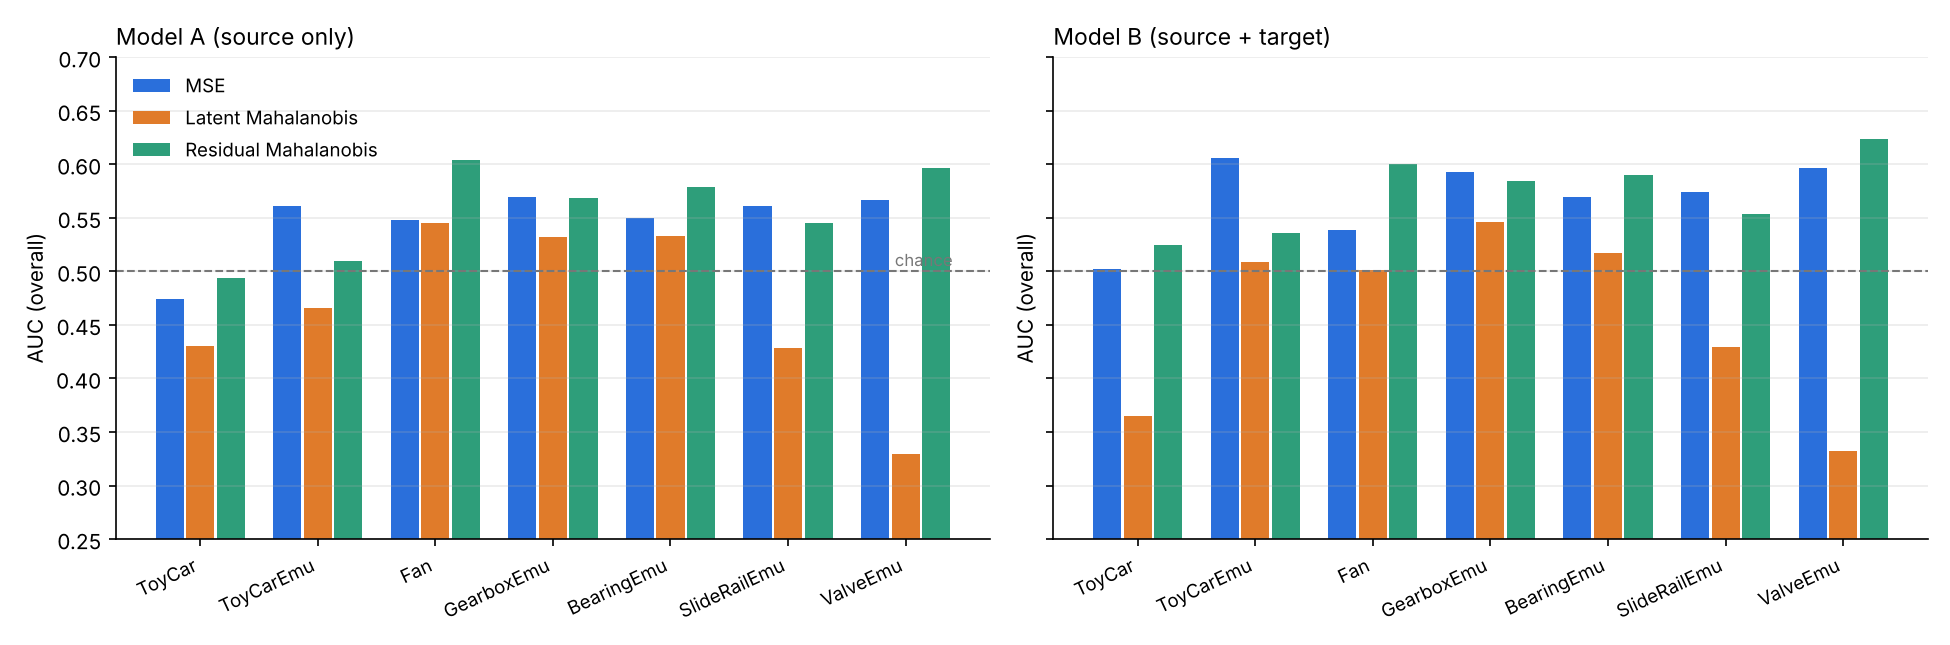
\includegraphics[width=\textwidth]{fig_auc_per_machine}
\caption{Overall AUC per machine type and scoring method; Model~A on the left, Model~B on the right.}
\label{fig:aucmach}
\end{figure}
\begin{figure}[!htb]\centering
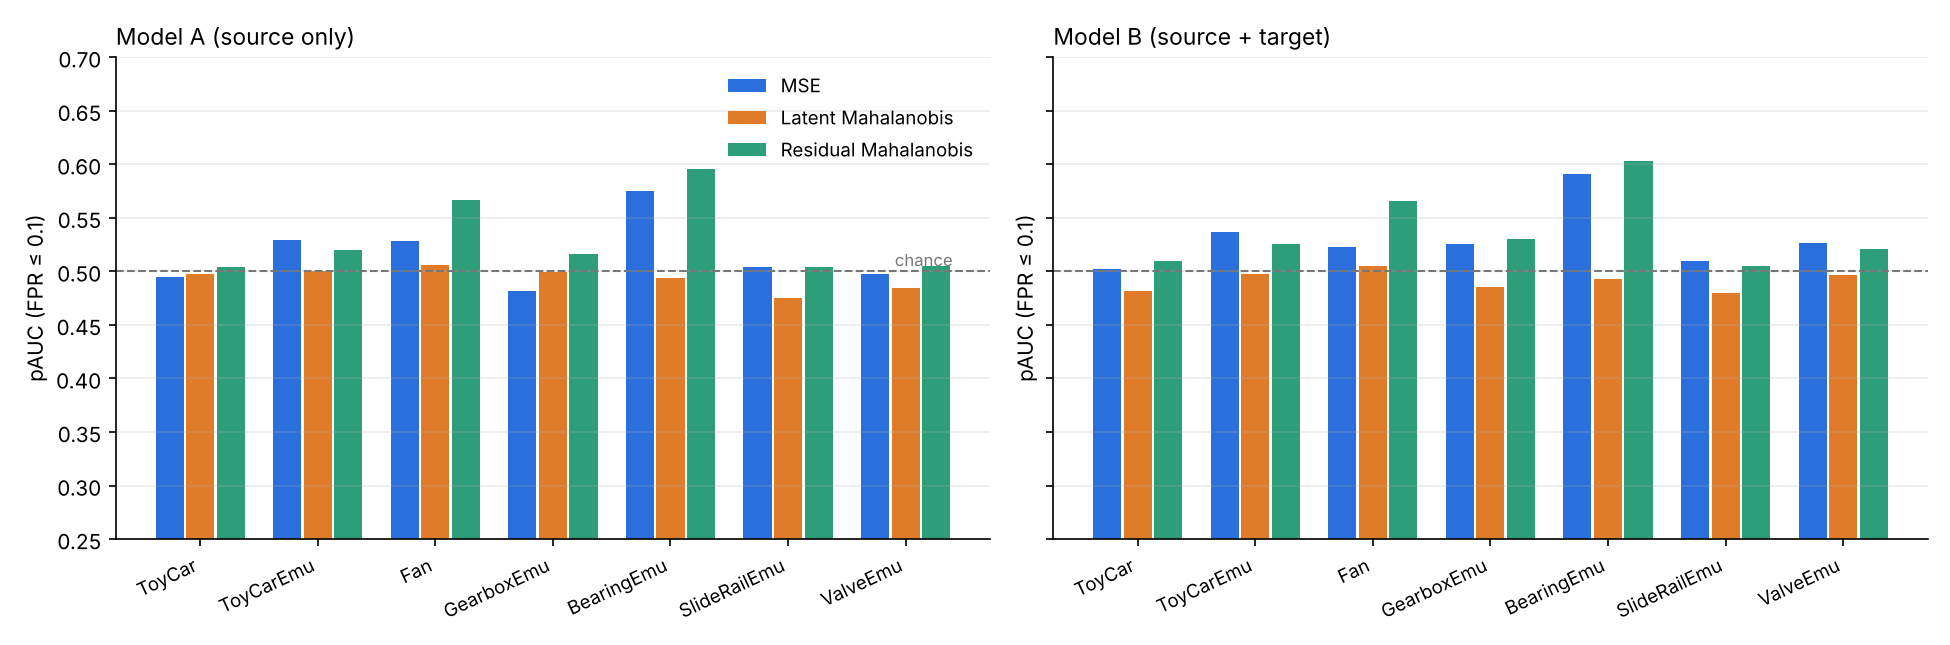
\includegraphics[width=\textwidth]{fig_pauc_per_machine}
\caption{Partial AUC (false-positive rate $\le 0.1$) per machine type and scoring method.}
\label{fig:paucmach}
\end{figure}
\begin{table}[!htb]
\centering
\caption{Best configuration per machine type by overall AUC.}
\label{tab:best}
\footnotesize
\renewcommand{\arraystretch}{1.18}
\begin{tabular}{lrrrr}
\toprule
Machine & Model & Scoring & AUC & pAUC \\
\midrule
BearingEmu & B & Res.\,Mah. & 0.590 & 0.603 \\
Fan & A & Res.\,Mah. & 0.604 & 0.567 \\
GearboxEmu & B & MSE & 0.593 & 0.525 \\
SlideRailEmu & B & MSE & 0.574 & 0.510 \\
ToyCar & B & Res.\,Mah. & 0.524 & 0.509 \\
ToyCarEmu & B & MSE & 0.605 & 0.537 \\
ValveEmu & B & Res.\,Mah. & 0.624 & 0.521 \\
\bottomrule
\end{tabular}
\end{table}

The highest overall AUC is reached on Valve (Emu) with Model~B and residual Mahalanobis scoring (0.624); ToyCar is the hardest machine, with 0.524 at best. For MSE and residual scoring the pAUC values lie between 0.48 and 0.60, which means that at low false-alarm rates the separation is modest for every machine. Latent Mahalanobis scoring is below 0.5 on four of the seven machines and falls to 0.33 on Valve (Emu), where it ranks anomalies systematically \emph{below} normal recordings.

\section{Model A versus Model B}
Adding the ten target recordings raises the overall AUC in 16 of the 21 machine-and-method combinations and the pAUC in 14 of 21. The improvements are small: the median AUC gain is about $+0.02$ for MSE and residual scoring, the largest is $+0.045$ on ToyCar (Emu) with MSE, and on Fan both scores decrease slightly. Averaged over machines, Model~B is ahead by 0.020 AUC with MSE and by 0.016 with residual Mahalanobis scoring. The direction is consistent, but with 200 test recordings per machine and one training run per model, differences of this size should be read as a tendency rather than as a demonstrated advantage.

\section{Source domain versus target domain}\label{sec:domain}
\begin{table}[!htb]
\centering
\caption{Model A: domain-specific metrics per machine type.}
\label{tab:domain_A}
\footnotesize
\renewcommand{\arraystretch}{1.18}
\resizebox{\textwidth}{!}{\begin{tabular}{lrrrrrrrrr}
\toprule
Machine & Scoring & AUC src & AUC tgt & P src & R src & F1 src & P tgt & R tgt & F1 tgt \\
\midrule
BearingEmu & MSE & 0.558 & 0.541 & 0.556 & 0.400 & 0.465 & 0.633 & 0.380 & 0.475 \\
BearingEmu & Lat.\,Mah. & 0.527 & 0.538 & 0.467 & 0.140 & 0.215 & 0.600 & 0.060 & 0.109 \\
BearingEmu & Res.\,Mah. & 0.581 & 0.577 & 0.576 & 0.380 & 0.458 & 0.633 & 0.380 & 0.475 \\
Fan & MSE & 0.620 & 0.476 & 0.889 & 0.160 & 0.271 & 0.400 & 0.040 & 0.073 \\
Fan & Lat.\,Mah. & 0.496 & 0.595 & 0.800 & 0.080 & 0.145 & 0.333 & 0.020 & 0.038 \\
Fan & Res.\,Mah. & 0.568 & 0.640 & 0.929 & 0.260 & 0.406 & 0.500 & 0.020 & 0.038 \\
GearboxEmu & MSE & 0.703 & 0.436 & 0.655 & 0.380 & 0.481 & 0.537 & 0.580 & 0.558 \\
GearboxEmu & Lat.\,Mah. & 0.554 & 0.509 & 0.375 & 0.060 & 0.103 & 0.500 & 0.080 & 0.138 \\
GearboxEmu & Res.\,Mah. & 0.657 & 0.479 & 0.773 & 0.340 & 0.472 & 0.523 & 0.460 & 0.489 \\
SlideRailEmu & MSE & 0.660 & 0.463 & 0.625 & 0.400 & 0.488 & 0.511 & 0.480 & 0.495 \\
SlideRailEmu & Lat.\,Mah. & 0.417 & 0.439 & 0.125 & 0.020 & 0.034 & 0.000 & 0.000 & 0.000 \\
SlideRailEmu & Res.\,Mah. & 0.665 & 0.426 & 0.643 & 0.360 & 0.462 & 0.458 & 0.440 & 0.449 \\
ToyCarEmu & MSE & 0.777 & 0.345 & 0.569 & 0.580 & 0.574 & 0.505 & 1.000 & 0.671 \\
ToyCarEmu & Lat.\,Mah. & 0.464 & 0.467 & 0.625 & 0.100 & 0.172 & 0.444 & 0.080 & 0.136 \\
ToyCarEmu & Res.\,Mah. & 0.759 & 0.260 & 0.519 & 0.540 & 0.529 & 0.500 & 1.000 & 0.667 \\
ToyCar & MSE & 0.713 & 0.236 & 0.476 & 0.400 & 0.435 & 0.495 & 0.980 & 0.658 \\
ToyCar & Lat.\,Mah. & 0.463 & 0.398 & 0.400 & 0.080 & 0.133 & 0.375 & 0.060 & 0.103 \\
ToyCar & Res.\,Mah. & 0.763 & 0.225 & 0.571 & 0.640 & 0.604 & 0.500 & 1.000 & 0.667 \\
ValveEmu & MSE & 0.577 & 0.557 & 0.250 & 0.040 & 0.069 & 0.636 & 0.140 & 0.230 \\
ValveEmu & Lat.\,Mah. & 0.391 & 0.267 & 0.250 & 0.020 & 0.037 & 0.400 & 0.040 & 0.073 \\
ValveEmu & Res.\,Mah. & 0.579 & 0.615 & 0.500 & 0.140 & 0.219 & 0.625 & 0.200 & 0.303 \\
\bottomrule
\end{tabular}}
\end{table}
\begin{table}[!htb]
\centering
\caption{Model B: domain-specific metrics per machine type. Precision, recall and F1 are computed within each domain at the calibrated threshold.}
\label{tab:domain_B}
\footnotesize
\renewcommand{\arraystretch}{1.18}
\resizebox{\textwidth}{!}{\begin{tabular}{lrrrrrrrrr}
\toprule
Machine & Scoring & AUC src & AUC tgt & P src & R src & F1 src & P tgt & R tgt & F1 tgt \\
\midrule
BearingEmu & MSE & 0.571 & 0.568 & 0.545 & 0.360 & 0.434 & 0.633 & 0.380 & 0.475 \\
BearingEmu & Lat.\,Mah. & 0.505 & 0.529 & 0.583 & 0.140 & 0.226 & 0.333 & 0.040 & 0.071 \\
BearingEmu & Res.\,Mah. & 0.586 & 0.594 & 0.581 & 0.360 & 0.444 & 0.679 & 0.380 & 0.487 \\
Fan & MSE & 0.604 & 0.474 & 0.778 & 0.140 & 0.237 & 0.333 & 0.040 & 0.071 \\
Fan & Lat.\,Mah. & 0.440 & 0.563 & 0.500 & 0.100 & 0.167 & 0.500 & 0.020 & 0.038 \\
Fan & Res.\,Mah. & 0.560 & 0.640 & 0.929 & 0.260 & 0.406 & 0.500 & 0.020 & 0.038 \\
GearboxEmu & MSE & 0.683 & 0.502 & 0.630 & 0.340 & 0.442 & 0.565 & 0.520 & 0.542 \\
GearboxEmu & Lat.\,Mah. & 0.557 & 0.535 & 0.222 & 0.040 & 0.068 & 0.667 & 0.080 & 0.143 \\
GearboxEmu & Res.\,Mah. & 0.653 & 0.515 & 0.773 & 0.340 & 0.472 & 0.523 & 0.460 & 0.489 \\
SlideRailEmu & MSE & 0.669 & 0.479 & 0.625 & 0.400 & 0.488 & 0.521 & 0.500 & 0.510 \\
SlideRailEmu & Lat.\,Mah. & 0.427 & 0.431 & 0.143 & 0.020 & 0.035 & 0.167 & 0.020 & 0.036 \\
SlideRailEmu & Res.\,Mah. & 0.670 & 0.436 & 0.667 & 0.360 & 0.468 & 0.469 & 0.460 & 0.465 \\
ToyCarEmu & MSE & 0.771 & 0.440 & 0.580 & 0.580 & 0.580 & 0.521 & 1.000 & 0.685 \\
ToyCarEmu & Lat.\,Mah. & 0.533 & 0.485 & 0.625 & 0.100 & 0.172 & 0.300 & 0.060 & 0.100 \\
ToyCarEmu & Res.\,Mah. & 0.755 & 0.316 & 0.523 & 0.460 & 0.489 & 0.500 & 1.000 & 0.667 \\
ToyCar & MSE & 0.673 & 0.330 & 0.474 & 0.360 & 0.409 & 0.500 & 0.860 & 0.632 \\
ToyCar & Lat.\,Mah. & 0.520 & 0.210 & 0.333 & 0.060 & 0.102 & 0.387 & 0.240 & 0.296 \\
ToyCar & Res.\,Mah. & 0.733 & 0.315 & 0.551 & 0.540 & 0.545 & 0.500 & 1.000 & 0.667 \\
ValveEmu & MSE & 0.600 & 0.592 & 0.636 & 0.140 & 0.230 & 0.706 & 0.240 & 0.358 \\
ValveEmu & Lat.\,Mah. & 0.414 & 0.249 & 0.429 & 0.060 & 0.105 & 0.455 & 0.100 & 0.164 \\
ValveEmu & Res.\,Mah. & 0.596 & 0.652 & 0.643 & 0.180 & 0.281 & 0.688 & 0.220 & 0.333 \\
\bottomrule
\end{tabular}}
\end{table}
\begin{figure}[!htb]\centering
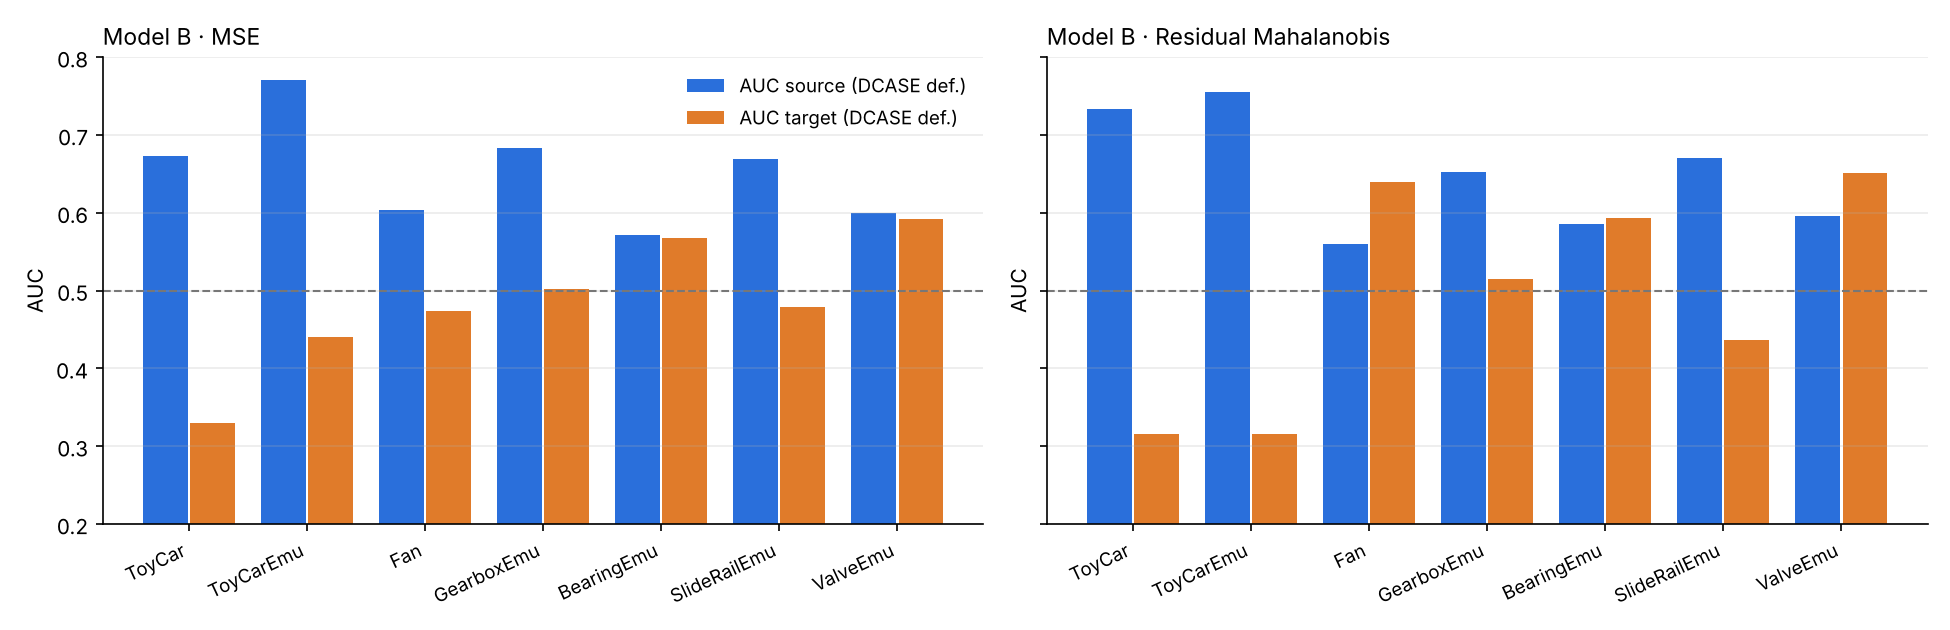
\includegraphics[width=\textwidth]{fig_domain_modelB}
\caption{Model~B: source-domain and target-domain AUC (DCASE definition) per machine, for MSE and residual Mahalanobis scoring.}
\label{fig:domain}
\end{figure}

Source-domain AUCs for MSE and residual scoring lie between 0.57 and 0.74, target-domain AUCs mostly between 0.38 and 0.55, and for several machines below 0.5. A target AUC below 0.5 has a concrete meaning: normal target-domain recordings receive \emph{higher} scores than anomalous recordings. The change of recording conditions raises the reconstruction error of a perfectly healthy target clip by more than a fault raises it, so the detector reacts to the environment rather than to the machine. Model~B narrows this gap, its average target AUC is 0.48 to 0.50 against 0.44 to 0.46 for Model~A, but ten recordings are not enough to close it.

\section{Decision rates and the cost of training-set calibration}\label{sec:rates}
\begin{table}[!htb]
\centering
\caption{Decision rates on the pooled test sets (1400 normal and 1400 anomalous recordings) at the Gamma 90th-percentile threshold fitted on training-set scores. A false-positive rate above 0.10 on normal test recordings quantifies the optimism of training-set calibration.}
\label{tab:rates}
\footnotesize
\renewcommand{\arraystretch}{1.18}
\begin{tabular}{lrrrrr}
\toprule
Model & Scoring & FPR normals & TPR anomalies & FPR src normals & FPR tgt normals \\
\midrule
A & Lat.\,Mah. & 0.086 & 0.060 & 0.094 & 0.077 \\
A & MSE & 0.363 & 0.426 & 0.254 & 0.471 \\
A & Res.\,Mah. & 0.359 & 0.440 & 0.246 & 0.471 \\
B & Lat.\,Mah. & 0.114 & 0.077 & 0.103 & 0.126 \\
B & MSE & 0.337 & 0.419 & 0.240 & 0.434 \\
B & Res.\,Mah. & 0.340 & 0.431 & 0.217 & 0.463 \\
\bottomrule
\end{tabular}
\end{table}
If training and unseen normal recordings had the same score distribution, a threshold at the 90th percentile of training scores would flag about 10\,\% of unseen normals. Table~\ref{tab:rates} shows what actually happens: with MSE and residual scoring 34 to 36\,\% of normal test recordings are flagged, 22 to 25\,\% in the source domain and 43 to 47\,\% in the target domain, while only 42 to 44\,\% of anomalous recordings are caught. This is the optimism of training-set calibration made visible, strongest where the domain shift is largest, and it is the reason the F1 values in Tables~\ref{tab:domain_A} and \ref{tab:domain_B} are low. The latent Mahalanobis thresholds behave differently (about 10\,\% false positives but only 6 to 8\,\% true positives) simply because that score hardly separates the classes at all.

\begin{figure}[!htb]\centering
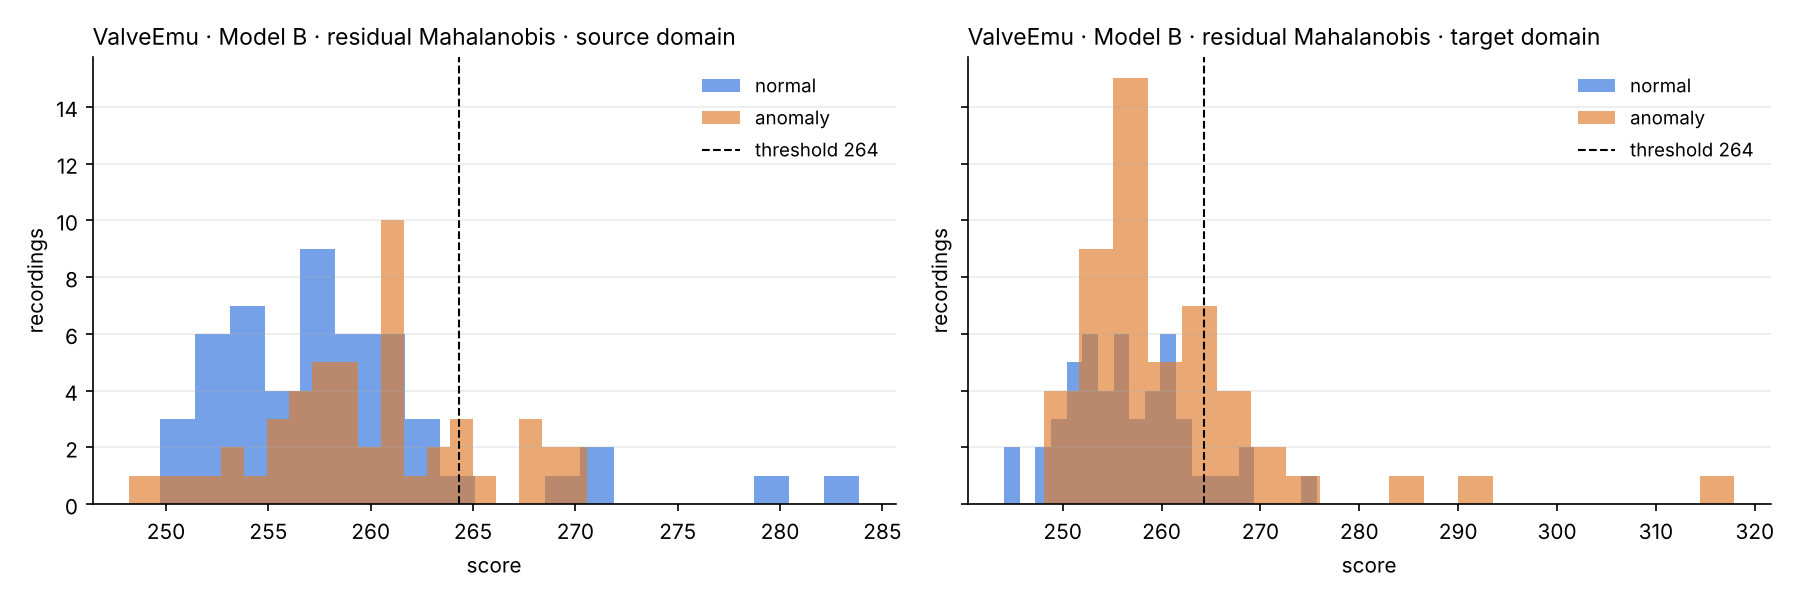
\includegraphics[width=\textwidth]{fig_scores_valve}
\caption{Valve (Emu), Model~B, residual Mahalanobis: score distributions of normal and anomalous test recordings with the calibrated threshold; source domain on the left, target domain on the right. In the target domain many normal recordings lie above the threshold.}
\label{fig:valve}
\end{figure}

\section{Best-performing combination}
On the actual data the best average configuration is \textbf{Model~B with residual Mahalanobis scoring}: AUC 0.573, pAUC 0.537, source AUC 0.650, target AUC 0.496. Model~B with MSE follows closely (0.568, 0.531, 0.653, 0.484). The margin between the two is within what seven machines and 200 test clips each can resolve, so the fair conclusion is that residual-space Mahalanobis scoring is at least as good as reconstruction MSE on this data, not that it is clearly better.

\chapter{Streamlit Application}\label{ch:app}
\section{What the application does}
The Streamlit application, \texttt{app.py}, offers a small interface in which the user chooses a machine type, one of the two models and one of the three scoring methods, uploads a WAV file and presses \emph{Analyse}. The application loads the corresponding checkpoint and Mahalanobis statistics from the handover folder, computes the score with \texttt{dcase\_part1\_lib}, reads the matching threshold from the Part~2 results and displays the score, the threshold, the number of analysed windows and a NORMAL or ABNORMAL decision. Because it imports the same module and the same files as the evaluation scripts, a recording analysed in the application receives exactly the score and decision recorded for it in the prediction files. The interface also shows a short caption warning that the thresholds were calibrated on training recordings and may be optimistic.

\section{Verification status}
During the final audit the application's inference path, from library import through checkpoint and statistics loading to scoring and threshold comparison, was executed programmatically on a WAV file for the Fan and ToyCar models, with both model variants and all three scoring methods. Every configuration produced finite scores and a decision; the first model load took about ten seconds and later analyses well under a second. That test used a synthetically generated noise recording, which every configuration flagged as abnormal, as one would hope. A test of the interactive interface on genuine recordings is not part of the evidence in the submission package; the execution instructions refer to screenshots kept in a separate shared document. The honest description of the application is therefore \emph{implemented and inference-verified}, not user-tested.

\chapter{Discussion and Limitations}\label{ch:discussion}
\section{What the results tell us}
Taken together, the numbers describe a detector that works in the conditions it was trained under and struggles when those conditions change. In the source domain the Autoencoder separates normal from anomalous sound with an AUC around 0.65, which is in the range one expects from a simple reconstruction-based baseline on recent DCASE data. In the target domain it is close to chance, and for several machines below it. The explanation is in the method itself. The Autoencoder is trained to rebuild normal source-domain windows and nothing else; any change in the acoustic surroundings increases its reconstruction error whether or not the machine is healthy. The ten target clips that Model~B sees are about one percent of its training data, enough to shift the standardisation statistics and the decoder a little, and that is what we observe: a small, mostly positive improvement that does not remove the problem.

The comparison of scoring methods is instructive. Residual-space Mahalanobis distance performed a little better than plain MSE because it reweights the 256 residual dimensions by how variable they are on normal data; bands that are always reconstructed poorly stop dominating the score. Latent-space distance failed because nothing in the training objective asks the bottleneck to be discriminative. Anomalous windows are reconstructed badly, but their codes are not unusual, so a distance measured in code space sees nothing.

\section{On threshold calibration}
The finding we consider most useful for anyone building on this work concerns the thresholds. The problem statement, like the official baseline, uses every normal recording for training, which leaves no independent normal recording for calibration. Fitting the threshold to training scores is then the only option, and Section~\ref{sec:rates} shows what it costs: in the target domain almost half of the healthy recordings are flagged. Threshold-free metrics such as AUC and pAUC are untouched by this, but any operating point is. The Part~1 notebook contains an optional cross-fitted calibration stage, in which fold models score recordings they never trained on, that would provide independent normal scores; we did not run it for the reported results, and it is the first thing we would do with more time.

\section{Limitations}
\begin{enumerate}
  \item \textbf{No independent validation set.} All 990 or 1\,000 normal recordings train each model. Overfitting cannot be assessed, and thresholds calibrated on training scores are optimistic (34 to 36\,\% false positives on normal test recordings instead of the intended 10\,\%).
  \item \textbf{Modest detection performance.} The best average AUC is 0.573 and target-domain AUC is near or below 0.5. The system is a baseline, not a detector one could deploy.
  \item \textbf{Not comparable with the official baseline.} Two-channel features, standardisation and the residual-space statistics mean that our numbers cannot be set against published baseline results.
  \item \textbf{Channel semantics.} The two channels are used with neutral labels. Nothing in this work establishes which physical microphone each channel represents, and a stereo file alone does not prove that two separate microphones were used.
  \item \textbf{One seed, one run.} Each model was trained once with seed 42. The variance between seeds was not measured, so differences of a few hundredths of AUC between configurations are not statistically established.
  \item \textbf{Selective scoring not evaluated.} Distances to the target-domain and all-training statistics were stored for every recording, but a selective score (the minimum over domain statistics, as in the official baseline) was not evaluated as a method of its own.
  \item \textbf{Application testing.} The interface is inference-verified but not user-tested on real recordings within the submitted evidence, and the application package omits the requirements file that its instructions mention.
  \item \textbf{Earlier prototype not retained.} An earlier ToyCar prototype trained with a 10\,\% hold-out was not available to the final pipeline run and is not included; all reported ToyCar models follow the \texttt{spec\_full} protocol.
\end{enumerate}

\chapter{Conclusion and Future Work}\label{ch:conclusion}
We set out to build, for all seven machine types of the DCASE 2026 Task~2 development set, an anomalous sound detector trained on normal recordings alone, and to run the three experiments the problem statement asked for. What exists at the end is a complete and reproducible pipeline: an audit of 8\,400 recordings, a shared two-channel log-Mel front end, fourteen trained Autoencoders, normal-distribution statistics for Mahalanobis scoring in two feature spaces, 2\,800 scored test recordings, 42 calibrated thresholds, full metric tables, verification reports and a demonstration application. A final audit recomputed every reported number from the raw score files and found no discrepancy.

The results themselves are sober. Residual-space Mahalanobis scoring with the source-plus-target model gave the best average performance (AUC 0.573, pAUC 0.537), reconstruction MSE was a close second, and scoring in the latent space was not useful. The source domain is handled reasonably; the target domain is not, and the ten target recordings help only a little. Calibrating thresholds on training scores, which the protocol leaves as the only option, proved clearly optimistic.

If we were to continue, we would, in this order: run the cross-fitted calibration stage that is already implemented, so that operating points rest on independent normal scores; evaluate selective Mahalanobis scoring with per-domain statistics and per-domain thresholds; repeat the training over several seeds to learn how much of the differences between configurations is noise; replace the dense Autoencoder with a representation trained to be discriminative, for example through attribute classification or contrastive pre-training, which recent challenge entries have found more robust to domain shift; and make explicit use of the two channels, now that the pipeline preserves both, through inter-channel features rather than simple concatenation.


\bibliographystyle{ieeetr}
\bibliography{references}
\addcontentsline{toc}{chapter}{References}

\appendix
\chapter{Technical Appendix}\label{app:tech}
\section{Project folder structure}\label{app:folders}
\begin{lstlisting}
DCASE_2026_PART1_COMPLETE/
  Dataset_Audit/            archive_structure.json, dataset_audit.csv (8400 rows), dataset_summary.json,
                            dataset_file_manifest.csv, dataset_integrity_report.md, per-machine files
  Preprocessing/            preprocessing_code/dcase_part1_lib.py, preprocessing_configs/<m>_*.json|npz
  Models/<m>/Source_Only|Source_Target/  <variant>_autoencoder.pth, *_model_config.json,
                            *_COMPLETE.json, TRAINING_PROTOCOL.txt, epoch_NNN.pth snapshots
  Training_Histories/       <m>_<variant>_training_history.csv, ALL_MACHINES_training_summary.csv
  Loss_Curves/              per-model and per-machine PNG, ALL_MACHINES_loss_curves.png
  Mahalanobis_Statistics/<m>/  <variant>_<group>_mahalanobis_stats.npz (groups: source_train,
                            target_train, all_train), <variant>_mahalanobis_report.json
  Configurations/           common_config.json, environment.json, pipeline_state.json
  Verification_Reports/     <m>_verification.md/.csv, ALL_MACHINES_verification_summary.csv
  Handover/ and DCASE_2026_PART1_COMPLETE_HANDOVER.zip (225 files, 55.3 MB)
Part2_Results/
  Test_Scores/              2800 rows: mse_score and latent/residual Mahalanobis to 3 groups
  Calibration_Scores/       14000 rows of training-normal scores
  Thresholds/               all_machine_thresholds.csv (42 rows, Gamma fit, 90th percentile)
  Binary_Predictions/       8400 rows (2800 recordings x 3 methods)
  Metrics/                  all_machine_metrics.csv (42 rows), Comparisons/, Graphs/
\end{lstlisting}

\section{Common configuration}
\begin{lstlisting}
sample_rate 16000, n_fft 1024, hop_length 512, n_mels 128, context_frames 5, power 2.0,
channel_mode "concat", normalise true, window_stride 1, epochs 100, batch_size 256,
learning_rate 0.001, seed 42, val_fraction 0.0, early_stop_patience null, split_protocol "spec_full"
\end{lstlisting}

\section{Model definition (from \texttt{dcase\_part1\_lib.py})}
\begin{lstlisting}[language=Python]
def dense_block(i, o):
    return nn.Sequential(nn.Linear(i, o), nn.BatchNorm1d(o, momentum=0.01, eps=1e-3), nn.ReLU())

class DCASEAutoencoder(nn.Module):
    def __init__(self, input_dim, hidden=128, latent=8, n_hidden=4):
        super().__init__()
        enc = [dense_block(input_dim, hidden)] + [dense_block(hidden, hidden) for _ in range(n_hidden-1)] \
              + [dense_block(hidden, latent)]
        dec = [dense_block(latent, hidden)] + [dense_block(hidden, hidden) for _ in range(n_hidden-1)] \
              + [nn.Linear(hidden, input_dim)]
        self.encoder, self.decoder = nn.Sequential(*enc), nn.Sequential(*dec)
    def forward(self, x):
        z = self.encoder(x)
        return self.decoder(z), z
\end{lstlisting}

\section{Scoring interface used by Part 2 and the application}
\begin{lstlisting}[language=Python]
model, ck = p1.load_checkpoint(".../Models/Fan/Source_Target/source_target_autoencoder.pth")
x   = p1.wav_to_model_input(wav_path, ck)        # (n_windows, 1280), standardised with ck statistics
res = p1.run_inference(model, x)                 # reconstruction, latent (n, 8), window_mse, residual
S   = p1.load_mahalanobis_stats(".../Mahalanobis_Statistics/Fan/source_target_all_train_mahalanobis_stats.npz")
mse      = res["window_mse"].mean()
d_latent = p1.mahalanobis_sq(res["latent"], S["latent_mean"], S["latent_precision"]).mean()
d_resid  = p1.mahalanobis_sq(res["residual"].reshape(-1, 256), S["residual_mean"], S["residual_precision"]).mean()
\end{lstlisting}

\section{Checks performed in the final audit}
\begin{enumerate}
  \item Test-score files: 2\,800 rows, 200 per machine and model; domain and label columns agree with the file names; window counts agree with clip durations (309, 340, 372); all scores finite and positive; per-machine files identical to the combined file.
  \item Calibration files: 14\,000 rows, all from \texttt{train/} normal recordings; no test file present.
  \item Thresholds: all 42 re-fitted from the calibration scores, maximum relative difference $2\times10^{-14}$.
  \item Predictions: 8\,400 rows; every score equals the corresponding entry of the score file and every decision follows from its threshold.
  \item Metrics: all 42 rows and the averages recomputed, maximum absolute difference $8\times10^{-17}$.
  \item Model and statistics files: 71 files byte-identical between the application package and the Part~1 handover archive.
  \item Verification summary: 14 of 14 models passed; pipeline state \texttt{COMPLETE} for all seven machines, handover \texttt{VERIFIED} (216 required files).
  \item Hardware: all 14 checkpoints record \texttt{device: cuda} with timestamps on 9~November~2026; the CPU record in \texttt{environment.json} belongs to the handover-verification session of 10~November.
\end{enumerate}


\end{document}
